%% SoftwareX Original Software Publication manuscript prepared from the
%% official SoftwareX OSP LaTeX template supplied by the authors.
%% The template class, metadata table, and five mandatory sections are retained.

\documentclass[preprint,12pt,a4paper]{elsarticle}

\usepackage{amssymb}
\usepackage{amsmath}
\usepackage{array}
\usepackage{booktabs}
\usepackage{float}
\usepackage{graphicx}
\usepackage{tabularx}
\usepackage{hyperref}
\hypersetup{hidelinks}
\newcolumntype{L}[1]{>{\raggedright\arraybackslash}p{#1}}
\newcolumntype{Y}{>{\raggedright\arraybackslash}X}
\setlength{\parindent}{0pt}
\setlength{\emergencystretch}{2em}

\journal{SoftwareX}

\begin{document}
\renewcommand{\labelenumii}{\arabic{enumi}.\arabic{enumii}}

\begin{frontmatter}

\title{MathHarnessAudit: Outcome-Linked Evidence Auditing for Mathematical Reasoning Agents}

\author[ytu]{Jianshuo Zhao\fnref{orcid-zhao}}
\ead{934508623@qq.com}
\author[ytu]{Weiqing Yan\corref{cor1}}
\ead{wqyan@tju.edu.cn}
\cortext[cor1]{Corresponding author.}
\fntext[orcid-zhao]{ORCID: \href{https://orcid.org/0009-0000-8086-4172}{0009-0000-8086-4172}.}

\address[ytu]{School of Computer and Control Engineering, Yantai University,
Yantai, China}

\begin{abstract}
MathHarnessAudit is an open-source Python package that converts heterogeneous
mathematical-agent traces into fidelity-labelled, outcome-linked evidence
records. It validates availability, provenance, decisions, latency, and cost;
applies conservative deterministic scoring; and reports dependence, joint
failure, repair/harm, utilization, repetition, and effective support with
explicit denominators and explicit counts of undefined bootstrap resamples.
Validation combines cross-platform release checks, a
150-episode descriptive audit of three systems, and a text-free public analysis
snapshot that regenerates the reported tables and figures byte for byte. The
audit exposed validator text repetition while retaining sparse and undefined
associations. The package supports evidence-structure analysis without ranking
systems or making causal architecture claims.
\end{abstract}

\begin{keyword}
mathematical reasoning agents \sep evidence provenance \sep error dependence
\sep tool verification \sep research software \sep reproducible evaluation
\end{keyword}

\end{frontmatter}

\section*{Required Metadata}

\section*{Current code version}

\begin{table}[H]
\centering
\small
\begin{tabularx}{\textwidth}{|l|L{4.8cm}|Y|}
\hline
\textbf{Nr.} & \textbf{Code metadata description} &
\textbf{Please fill in this column} \\
\hline
C1 & Current code version & 0.2.2 \\
\hline
C2 & Permanent GitHub link to code/repository used for this code version &
\url{https://github.com/abaiar/MathHarnessAudit/tree/v0.2.2} \\
\hline
C3 & Legal Code License & MIT \\
\hline
C4 & Code versioning system used & Git \\
\hline
C5 & Software code languages, tools, and services used & Python 3.10--3.12;
Pydantic, NumPy, pandas, SciPy, SymPy, Typer, Rich; optional PyArrow and
jsonschema; pytest, Ruff, uv, and GitHub Actions \\
\hline
C6 & Compilation requirements, operating environments \& dependencies &
Platform-independent Python wheel; dependencies are declared in
\texttt{pyproject.toml} and locked in \texttt{uv.lock}; CI covers
Ubuntu and Windows with Python 3.10 and 3.12 \\
\hline
C7 & If available link to developer documentation/manual & Versioned repository README,
CLI help, \texttt{examples/README.md}, adapter and migration tutorials,
troubleshooting guide, schemas, and synthetic fixtures under the C2 tag \\
\hline
C8 & Support email for questions & \url{wqyan@tju.edu.cn} \\
\hline
\end{tabularx}
\caption{Code metadata (mandatory).}
\label{tab:code-metadata}
\end{table}

\section{Motivation and significance}
\label{sec:motivation}

Mathematical-agent evaluations commonly reduce a run to a final answer and a
correctness bit. That summary is useful for benchmarking, but it hides the
mechanism that produced the answer. A three-agent majority may represent three
distinct checks, three correlated samples from one failure mode, or one answer
copied twice. Executable evidence may support an upstream answer, contradict
it, remain unused, fail, or never be requested. These trajectories can share
the same final score while supporting different conclusions about reliability.

Existing software addresses adjacent layers. OpenTelemetry conventions and
AgentTrace structure execution telemetry
\cite{opentelemetry2026genai,alsayyad2026agenttrace}; TRACER and LEDGER connect
claims to tool evidence or execution graphs \cite{yu2026tracer,kim2026ledger};
and $A^2E$ and MASEval evaluate harnesses or multi-agent systems
\cite{wang2026a2e,emde2026maseval}. MathGoal is the closest publication-form
comparator in mathematical workflow software \cite{hong2026mathgoal}.
AgentAuditor and ThinkBooster instead alter inference-time reasoning or scaling
\cite{yang2026agentauditor,smirnov2026thinkbooster}. Analyses of judge panels,
co-failure, correlation ceilings, and verifier cascades motivate measuring
dependence rather than assuming that nominally additional votes are independent
\cite{kohli2026ninejudges,chen2026cofailure,bay2026correlationceiling,
han2026verifiercascades}.

These projects overlap at the level of ``agent auditing'' but expose different
measurement objects. Table~\ref{tab:positioning} states the functional boundary
rather than claiming priority.

\begin{table}[!ht]
\centering
\small
\begin{tabularx}{\textwidth}{@{}L{2.6cm}L{4.1cm}Y@{}}
\toprule
\textbf{Software} & \textbf{Primary object} & \textbf{Difference from this package} \\
\midrule
MathGoal & Mathematical solving routes and prediction artifacts & Constructs
workflows; MathHarnessAudit measures evidence availability, error association,
and recorded selection after a run \\
$A^2E$/MASEval & Harness capability or system-level evaluation & Broader task and
system comparison; no identical domain scoring/denominator contract is claimed \\
TRACER/\allowbreak LEDGER & Claim-to-evidence provenance and execution review & Rich claim or
workflow traceability; not the same registered mathematical error estimands \\
AgentTrace/\allowbreak OTel & General execution observability & Supplies telemetry that can
feed an adapter, but not outcome-linked mathematical audit statistics \\
\bottomrule
\end{tabularx}
\caption{Capability-level positioning based on the cited primary descriptions.
``Different'' means not a stated primary contract, not that extension is
impossible.}
\label{tab:positioning}
\end{table}

A practical measurement gap remains. A trace can establish that an agent or
tool ran without establishing whether its output was scorable, correct,
provenance-distinct, jointly wrong with another source, or used in the final
decision. MathHarnessAudit fills this gap with a portable, outcome-linked data
contract and a tested path from native traces to publication artifacts. The
software leaves the audited harness unchanged, keeps unavailable fields
unavailable, and binds each estimate to a registered population and denominator.
It is intended for agent developers comparing revisions, evaluators auditing
reported systems, and researchers studying whether nominal redundancy
corresponds to distinct operational evidence. It is a measurement package, not
a new aggregation policy; adaptive routing and causal optimization are outside
this article.

The experimental workflow is direct. A user exports a native trace, selects a
built-in adapter or implements the documented adapter protocol, validates the
canonical episodes, applies a registered scoring route, and generates audit and
publication outputs. A provider-free fixture demonstrates the same workflow
without model credentials.

\section{Software description}
\label{sec:software}

\subsection{Software architecture}

The package comprises five layers (Fig.~\ref{fig:architecture}). Fidelity-aware adapters first translate traces
from ICMA, MathRouterAgent, MathGoal, canonical JSON, or a conservative
OpenTelemetry bridge. Each adapter declares observable fields and must not
invent tool calls, dependencies, or decisions. Fidelity levels distinguish
complete decision/provenance traces from partial and final-only records.

The canonical contract represents an episode as typed sources, observations,
evidence items, decisions, provenance edges, final output, latency and cost,
plus an audit-only reference answer. Availability is data rather than a
preprocessing nuisance: \texttt{not\_called}, \texttt{no\_vote},
\texttt{failed}, \texttt{timeout}, \texttt{abstain}, and
\texttt{not\_observable} remain distinct from an incorrect answer. Validators
check identifiers, cross-references, temporal relations, and isolation of the
reference answer before analysis.

The scorer normalizes supported answer forms and applies exact, rational-numeric,
registered categorical, and restricted symbolic-equivalence rules. Unsafe symbolic inputs are
rejected. Every produced target terminates as correct, incorrect, abstain, or
unscorable; unsupported mathematics is not silently guessed. Optional human
annotations remain separate and never overwrite the deterministic result.

The audit engine reports source availability before outcome association. For
paired binary error indicators, let $n_{11}$ denote both sources wrong,
$n_{10}$ only the first wrong, $n_{01}$ only the second wrong, and $n_{00}$ both
correct. The package reports the complete table and
\begin{equation}
\phi=\frac{n_{11}n_{00}-n_{10}n_{01}}
{\sqrt{(n_{11}+n_{10})(n_{01}+n_{00})(n_{11}+n_{01})(n_{10}+n_{00})}},
\end{equation}
leaving $\phi$ undefined when an error marginal has zero variance. For a source-
type pair with a variable number of candidates, each informative episode first
contributes four within-episode cell proportions $p_{ij}^{(e)}$; the primary
cells are $\bar p_{ij}=E_e[p_{ij}^{(e)}]$, and $\phi$ is evaluated on
$\bar p_{ij}$. Pooled integer cells are retained only as a sensitivity view.
Episode-cluster bootstrap resamples episodes and preserves within-episode
dependence. Because zero error marginals can make $\phi$ undefined, every result
reports requested, defined, and undefined replicate counts. The exported
2.5--97.5 percentile range is conditional on the defined replicates and is an
instability diagnostic, not a coverage-guaranteed 95\% confidence interval. The
all-wrong probability is computed only on complete cases, while a separate
operational measure asks whether any correct support was produced on every
registered episode. For an explicitly exchangeable repeated-source model,
variance-equivalent support is
\begin{equation}
N_{\mathrm{eff}}(k,\rho)=\frac{k}{1+(k-1)\rho},
\end{equation}
and is labelled model-based rather than a literal vote count. Directed
transitions distinguish repair opportunity from realized repair and harm
opportunity from realized harm. Recorded source selection is kept separate from
a final-text-match proxy.

Finally, the publication layer writes normalized JSON/JSONL or optional
Parquet, standalone HTML, CSV tables, accessible SVG figures, and self-hashed
manifests. It checks registered system-by-stratum panels, source pairs,
bootstrap settings, and denominator definitions, and refuses missing panels or
nonempty output destinations.

\begin{figure}[!ht]
\centering
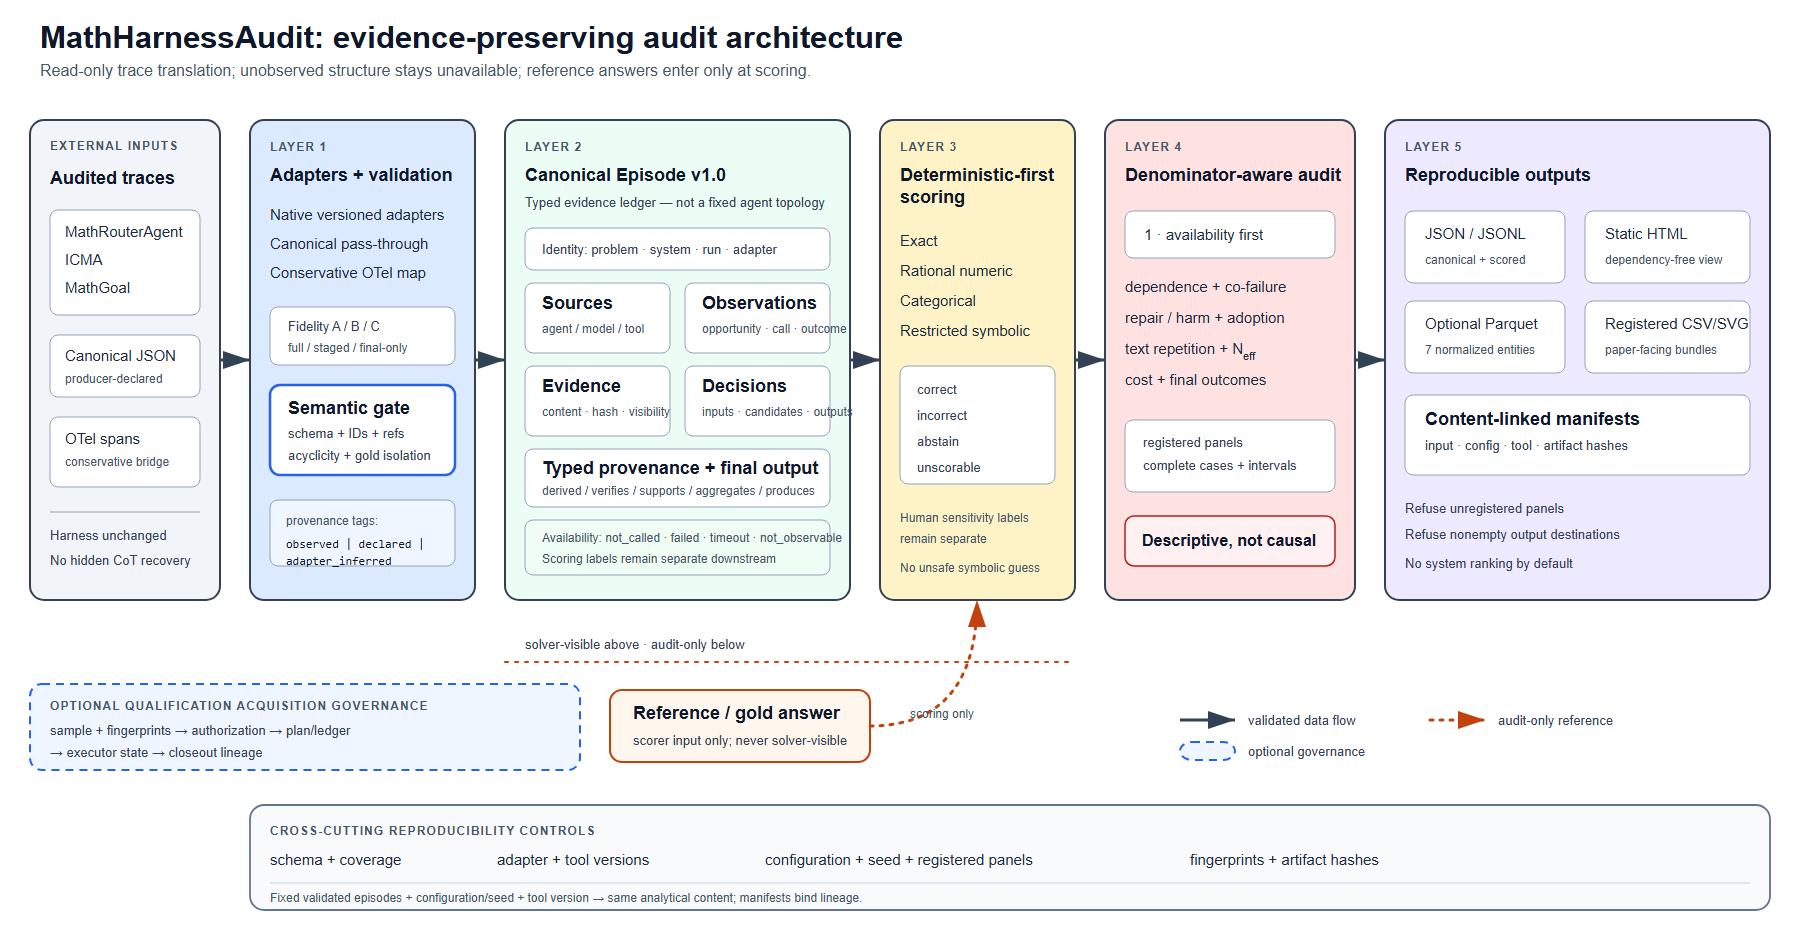
\includegraphics[width=0.98\textwidth]{figures/software_architecture.png}
\caption{Five-layer, read-only audit architecture. Fidelity-aware adapters and
semantic validation convert native traces into canonical episodes; reference
answers cross only the audit-only scoring boundary, and reported transitions
remain descriptive rather than causal. OpenAI Codex assisted the diagram layout;
the labels and connections were checked against the executable interfaces and
statistical contract. The hosted service was accessed in September 2026; a fixed
model build identifier was not exposed.}
\label{fig:architecture}
\end{figure}

\subsection{Software functionalities and interface boundary}

The command-line interface exposes six functional groups:
\texttt{mathaudit} \texttt{ingest} converts traces; \texttt{validate} checks canonical
episodes; \texttt{coverage} reports what an adapter can observe;
\texttt{score} applies a scoring route; and \texttt{report} or
\texttt{publish} generates artifacts. The stable public interface is the
canonical schema, not a private directory layout.

A previously unseen system can use direct canonical export, mapped
OpenTelemetry spans, or a small versioned adapter. The adapter protocol requires
a declared version and fidelity level, fixtures, and coverage expectations.
Lower-fidelity traces can still support availability or cost summaries;
analyses requiring unobserved provenance, dependence, repair, or adoption are
disabled rather than approximated. The package does not reconstruct hidden
chain-of-thought, equate absence with failure, or infer architecture from a
directory name. Table~\ref{tab:adapters} makes this reuse boundary explicit.

\begin{table}[!ht]
\centering
\small
\begin{tabularx}{\textwidth}{@{}L{3.0cm}L{3.2cm}L{2.1cm}Y@{}}
\toprule
\textbf{Route} & \textbf{Accepted input} & \textbf{Maximum fidelity} &
\textbf{Unsupported inference} \\
\midrule
MathRouter\allowbreak Agent /\allowbreak ICMA & Observed staged traces & B & Missing parentage,
selection, or stage cost is not inferred \\
MathGoal & Full \texttt{SolveResult} / compact output & A / C & Final-only output
cannot support dependence, repair/harm, or adoption \\
Canonical JSON & Producer-declared canonical episode & Declared & Fields absent
from the validated record remain unavailable \\
OpenTelemetry & Mapped agent spans & B or C & Mathematical evidence is not
inferred from generic spans \\
\bottomrule
\end{tabularx}
\caption{Adapter routes and explicit analysis boundaries.}
\label{tab:adapters}
\end{table}

\section{Illustrative examples}
\label{sec:examples}

The repository includes a provider-free ICMA-shaped fixture. From a source
checkout, a user runs:
\begin{verbatim}
uv run --extra dev python examples/run_demo.py \
  --output-dir tmp/fixture-demo
\end{verbatim}
The command adapts the synthetic trace, validates references and reference-
answer isolation, scores supported answers, audits the reasoner and Python
source, and writes \path{report.json}, \path{manifest.json}, and a
standalone \path{index.html}. Optional Parquet export creates seven normalized
tables for episodes, sources, source observations, evidence, decisions,
provenance edges, and labels.

The report first states whether each registered source was eligible, called,
and produced evidence. It then displays labels and paired $2\times2$ cells.
With one tutorial episode, phi is normally undefined because an error marginal
has zero variance. This is expected: the example demonstrates data flow and
denominator semantics rather than an empirical conclusion. The same commands
apply to a new system once its adapter emits canonical episodes.

\begin{figure}[!ht]
\centering
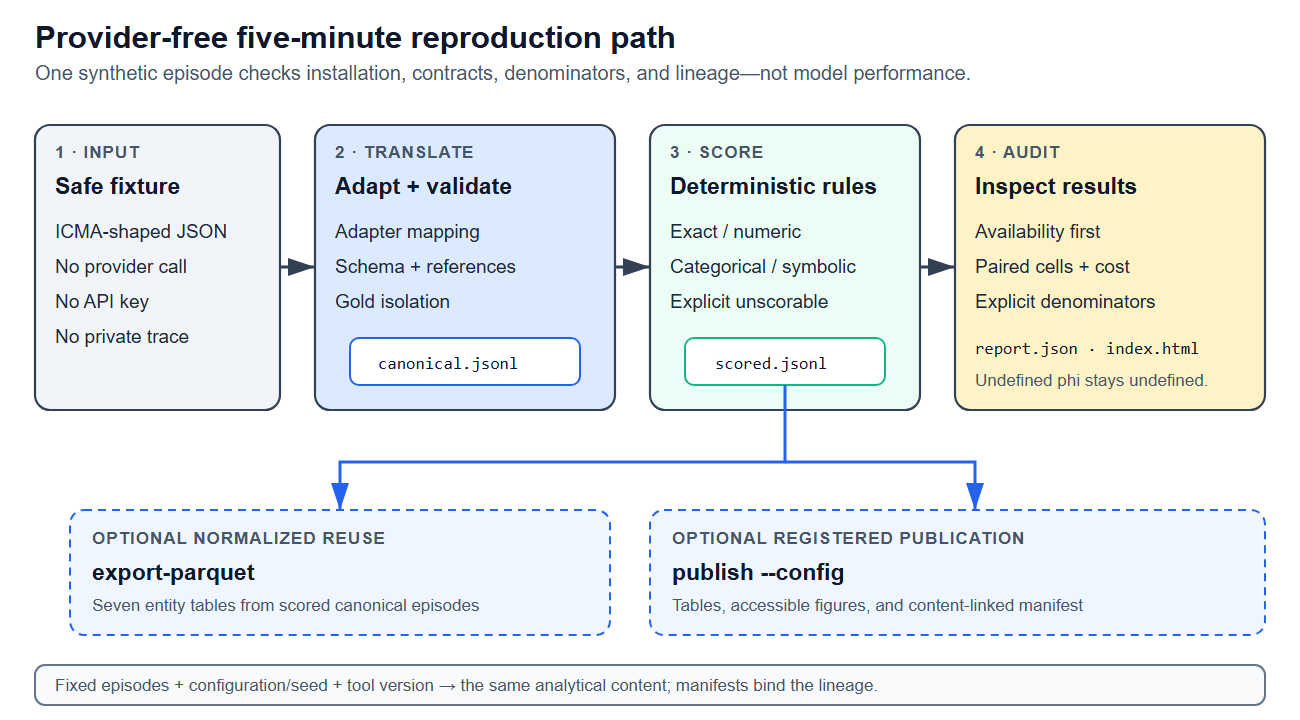
\includegraphics[width=0.95\textwidth]{figures/five_minute_workflow.png}
\caption{Provider-free core demonstration and optional output branches.
Reporting, Parquet export, and registered publication consume the scored
canonical episodes; the one-episode fixture demonstrates behavior and lineage,
not model performance. OpenAI Codex assisted the diagram layout; the flow was
checked against the provider-free fixture commands. The hosted service
was accessed in September 2026; a fixed model build identifier was not exposed.}
\label{fig:workflow}
\end{figure}

\section{Impact}
\label{sec:impact}

\subsection{Software validation and reproducibility}

Validation targets four reuse risks: semantic corruption during conversion,
incorrect mathematical labels or denominators, installation/platform failures,
and private-data leakage. Tests exercise canonical invariants, every built-in
adapter, scoring oracles, adversarial symbolic inputs, missingness rules, CLI
workflows, qualification lineage, publication output, and distribution hygiene.
OpenAI Codex assisted the v0.2.2 repository audit and implementation. Authors
retain responsibility for the submitted version; deterministic tests,
independent hash checks, and clean installation runs---rather than model
self-assessment---are the verification mechanisms reported here.

The v0.2.2 public candidate passed 150 public tests and Ruff in the development
workspace.
Source and wheel distributions built successfully, and a clean wheel environment
passed CLI, schema-export, validation, and provider-free fixture smoke checks.
The CI definition covers Ubuntu and Windows with Python 3.10 and 3.12 and audits
dependencies on the Linux/Python 3.12 leg. Boundary checks reject raw prompt,
answer, rationale, request-identifier, credential-shaped, and local-path fields
from the public aggregate analysis. MIT licensing appears in package metadata,
root license files, and public Python SPDX headers.

The repository now includes the exact configuration, a self-hashed text-free
analysis snapshot, generated tables/figures, and a claim ledger. The command
\texttt{qualification-reproduce-check} regenerates the publication bundle in a
temporary directory and requires every byte to match the committed reference;
\texttt{paper/verify\_claims.py} binds each registered manuscript number to one
or more uniquely selected CSV rows. Table~\ref{tab:quality} summarizes the
candidate checks.

\begin{table}[!ht]
\centering
\small
\begin{tabularx}{\textwidth}{@{}L{3.3cm}L{3.2cm}Y@{}}
\toprule
\textbf{Validation target} & \textbf{Observed result} & \textbf{Boundary} \\
\midrule
Stable public suite & 150 public tests; Ruff passed & Candidate source tree \\
Built distributions & Source and wheel build passed & Clean-wheel smoke verified \\
Aggregate release boundary & Zero forbidden text, secret, request-ID, or local-path fields &
Does not publish restricted raw traces \\
Paper reproduction & All registered files regenerated byte-identically & Aggregate-analysis-to-artifact boundary \\
Claim ledger & Seven numerical claim groups passed & Exact CSV selectors and manuscript markers \\
Release CI gate & Ubuntu/\allowbreak Windows $\times$ Python 3.10/3.12 & The immutable release is published only after the tagged workflow passes \\
\bottomrule
\end{tabularx}
\caption{Software quality and reproducibility checks for candidate v0.2.2.}
\label{tab:quality}
\end{table}

\subsection{Descriptive reference audit}

The reference audit is an end-to-end validation case, not a leaderboard. It
contains 150 complete episodes: 50 per system, each split into 25 MATH-500
standard tasks and 25 Omni-MATH tasks with registered difficulty greater than
five \cite{hendrycks2021math,gao2024omnimath}. The systems used the same frozen
provider/model family under their native orchestration. Analysis panels,
denominators, and 10,000 requested
episode-cluster bootstrap replicates (seed 20260823) were fixed before outcome
inspection. System ranking and architecture-causality claims were disabled.

Unsupported answer forms remained explicitly unscorable rather than being
relabelled as wrong. Final-answer counts varied across panels but are not
treated as comparable rankings because scoreability and observability differed.
Private human-rating materials were excluded from the paper evidence base: no
human-derived label or agreement estimate is used below.

Dependence varied across observable cells. The only LLM--LLM cell meeting the
registered 20-episode precision threshold was MathGoal-standard: 22 episodes,
182 pair observations, and episode-balanced $\phi=-0.0061$. Of 10,000 requested
cluster-bootstrap draws, 6,439 were defined; their conditional 2.5--97.5
percentile range was $-0.0250$ to $-0.0061$. MathGoal-standard LLM--Python used
16 episodes and gave $\phi=0.2592$; 6,465/10,000 draws were defined, with
conditional range 0.1882--0.3974. ICMA-standard used 14 episodes and gave
$\phi=0.6794$; 6,486/10,000 draws were defined, with conditional range
0.4385--1.0000. Both latter cells remained flagged as imprecise. These ranges
have no asserted nominal coverage. Hard-stratum
cells used at most seven episodes. Other cells were structurally absent or had
zero-variance marginals. These data support neither a universal high-LLM-
correlation constant nor a universal Python-independence constant.
% claim-id:dependence-mathgoal-standard-llm-llm
% claim-id:dependence-mathgoal-standard-llm-python
% claim-id:dependence-icma-standard-llm-python

Complete-case and operational joint-failure denominators also differed. The
registered MathRouter three-source sets had no complete cases, while operational
no-correct-support counts were 7/25 standard and 22/25 hard. ICMA-standard had
zero all-wrong cases among 13 complete cases (exact 95\% interval 0--0.2471),
and ICMA-hard had one among four (0.0063--0.8059). Repair/harm cells were sparse:
ICMA-standard had one harm opportunity and no realized harm; ICMA-hard had one
upstream-wrong/checker-scorable episode but no repair opportunity. These are
descriptive transitions, not causal tool effects.
% claim-id:cofailure-mathrouter
% claim-id:cofailure-icma
% claim-id:transitions-icma-sparse

The clearest structural observation was exact repetition. The ICMA validator
repeated the normalized reasoner text in 23/24 comparable standard episodes,
0.9583 (exact 95\% interval 0.7888--0.9989), and 19/23 hard episodes, 0.8261
(0.6122--0.9505). Exact repetition is narrower than semantic equivalence, but it
reveals redundancy that final accuracy and nominal agent count cannot show.
Undefined and sparse cells, including every undefined bootstrap draw, remain
visible in the exported tables.
% claim-id:repetition-icma

\begin{table}[!ht]
\centering
\small
\begin{tabularx}{\textwidth}{@{}L{3.2cm}L{3.8cm}Y@{}}
\toprule
\textbf{Audit view} & \textbf{Illustrative observation} & \textbf{Interpretive boundary} \\
\midrule
Scoreability & Unsupported forms remain unscorable & Missingness is not changed
to error \\
Dependence & One LLM--LLM cell met the registered episode threshold & Sparse and
undefined cells prohibit universal constants \\
Joint failure & Complete-case and all-episode operational denominators diverged &
Missing sources are not silently counted as wrong \\
Repair/harm & Opportunities and realizations were rare & Observational data do
not identify causal tool value \\
Repetition & ICMA exact repeats: 23/24 standard; 19/23 hard & Text identity is not
semantic equivalence \\
\bottomrule
\end{tabularx}
\caption{Selected descriptive outputs from the 150-episode reference audit.}
\label{tab:audit}
\end{table}

\subsection{Research impact, limitations, and reuse}

MathHarnessAudit turns system-specific notebook work into a repeatable workflow.
Users can ask whether a source was available, inspect recorded parentage, see
how many complete cases support an association, distinguish opportunities from
realized final transitions, and compare nominal source count with model-based
effective support. The canonical, adapter, and OpenTelemetry routes provide a
shared audit vocabulary without modifying inference policies. Hash-linked
configuration and outputs make null, undefined, and sparse findings reproducible.

The software enables research questions that final-answer benchmarks cannot
address directly: whether nominally separate sources fail together, whether an
executable check contributes information beyond language-model samples,
whether contradictory evidence is selected, and which observability gaps make
these questions unidentified. It supplies variables, denominators, and
uncertainty rather than asserting a universal architecture effect. Versioned
CLI commands, a provider-free fixture, adapter tutorial, schemas, and buildable
wheel/source artifacts reduce integration cost. The public paper bundle adds a
second provider-free route: it verifies the release boundary, regenerates every
audit table and figure, and checks manuscript values without private data or
network access. No adoption, download, or widespread-use claim is made.

The reference audit is observational. Selective tool invocation confounds
transition and adoption rates, and causal tool-value claims require randomized
call/no-call assignment or a controlled fork. Deterministic equivalence does not
cover every proof or malformed answer. Exact repetition is not semantic
redundancy. Low-fidelity traces cannot recover hidden
decisions. The three systems differ in observability, 25 episodes per stratum
leave rare cells imprecise, and provider drift limits cost comparison. Private
prompts, responses, credentials, and restricted trajectories cannot be released.
The public aggregate therefore reproduces analysis-to-artifact computation but
cannot repeat provider calls or raw-answer scoring. These limitations are
represented as unavailable fields, fidelity labels, intervals, or explicit
nonclaims.

\section{Conclusions}
\label{sec:conclusions}

The package provides a reproducible path from heterogeneous mathematical-
agent traces to validated, outcome-linked evidence audits. Its contribution is
the tested integration of conservative mathematical scoring, availability-aware
denominators, provenance, dependence, joint failure, transition and adoption
accounting, and hash-linked publication outputs. The 150-episode reference audit
shows why these properties cannot be reconstructed from final accuracy or agent
count alone. Public code, schemas, fixtures, tests, tutorials, aggregate analysis
data, and hash-linked artifacts make the workflow inspectable and extensible. Controlled
causal evaluation and adaptive routing remain separate future work.

\section*{CRediT authorship contribution statement}

Conceptualization: Jianshuo Zhao. Methodology: Jianshuo Zhao and Weiqing Yan.
Software: Jianshuo Zhao. Validation: Jianshuo Zhao. Formal analysis: Jianshuo
Zhao. Investigation: Jianshuo Zhao. Data curation: Jianshuo Zhao. Writing --
original draft: Jianshuo Zhao. Writing -- review \& editing: Jianshuo Zhao and
Weiqing Yan. Visualization: Jianshuo Zhao. Supervision: Weiqing Yan. Project
administration: Jianshuo Zhao.

\section*{Funding}

This work received support through a research project led by Weiqing Yan. No
external funding agency or grant number is declared.

\section*{Declaration of competing interest}

The authors declare no known competing financial interests or personal
relationships that could have appeared to influence the work reported in this
paper.

\section*{Acknowledgements}

None.

\section*{Ethics statement}

This manuscript does not analyze or report human ratings, participant responses,
or identifiable personal data. Private human-rating and independent-reuse
records created during development are outside the paper evidence base and the
public release. The authors remain responsible for obtaining any institutional
determination required before reusing those records in future research.

\section*{Declaration of generative AI and AI-assisted technologies in the
manuscript preparation process}

% Submission gate: both authors must approve the exact final statement below.
During preparation of this work, the authors used OpenAI Codex (hosted service,
accessed August--September 2026; fixed model build identifier not exposed) to
assist with repository inspection, software
implementation and tests, literature discovery, diagram layout, and language and
structural editing. The frozen 150-episode model runs predated the v0.2.2
repository revision and were not regenerated by Codex. After using the tool, the
authors reviewed and edited the material, verified citations, software behavior,
analysis code, generated artifacts, and reported values, and take full
responsibility for the content of the article.

\section*{Data availability}

Code, schemas, synthetic fixtures, documentation, the text-free frozen analysis
snapshot, generated tables and figures, and the claim ledger accompany version
0.2.2 at \url{https://github.com/abaiar/MathHarnessAudit/tree/v0.2.2}. The public bundle
supports aggregate-analysis-to-artifact reproduction. API keys, provider request
identifiers, linkable attempt identifiers, real prompts and responses, hidden
reasoning, restricted benchmark rows, real trajectories, private linkage, and
annotator rationales remain private. Their absence prevents raw-run
re-execution and is not described as full open-data reproducibility.

\bibliographystyle{elsarticle-num}
\bibliography{references_final}

\section*{Current executable software version}

The submission candidate is version 0.2.2. It supports Python 3.10--3.12 and is
packaged as a source distribution and platform-independent wheel. From the
repository, users may run \texttt{python -m pip install -e ".[schema]"}; release
users may install \path{math_harness_audit-0.2.2-py3-none-any.whl} with
\texttt{python -m pip install}. Documentation and issue-based support are
available in the GitHub repository.

\end{document}
\endinput
